In this chapter we describe the overall structure digital back-end of the Q-Pix design as well as results prototype boards to test the design.
As described in previous chapters, the digital back-end of the Q-Pix readout relies on an array of ASICs (FPGAs, here), which we refer to here to as digital nodes.
Each digital node in the array is implemented as a lattice ice40UP5k FPGA.

This chapter is divided into two parts.
The first part we give a detailed description of the digital-system, and its requirements to successful in a Q-Pix based detector of DUNE scales.
The motivation here is to outline how the digital backend of Q-Pix based readout fits into the DUNE-FD LArTPC. 
The second part of this chapter is dedicated to the first evaluation boards developed and tested which are implemented in Lattice iCE40UP FGPAs~\citep{lattice_ice40up_datasheet}.
The second part also outlines the design of the PCB on which these FPGAs are implemented, as well as basic results of these FGPAs, which are motivated from the first part of this chapter.

The Lattice Semiconductor FPGAs \citep{lattice_ice40up_datasheet} were selected because of the small form factor, pin out, availability, as well as lower power consumption.
There are planned tests for future, but not presented here to indicate its viability of over-the-counter FPGAs in LArTPc. 
If such cheap and available FPGAs were shown to be reliable use in a LArTPC environment, that would greatly influence future detector development and selection for Q-Pix.

All results presented in this chapter are my own individual work.

\section{Digital Design Overview}

The digital system of the Q-Pix design begins at the collection of a recorded timestamp in response to the logic reset pulse sent from the integrating analog front-end.
When a reset occurs the data recorded are the reset values of each pixel, and the only data required for a full analysis of all reconstruction with a LArTPC are:

\begin{itemize}
    \item 32 bit timestamp
    \item Pixel X location ($\le 4$ bits)
    \item Pixel Y location ($\le 4$ bits)
    \item Pixel Mask ($\le 16$ bits)
\end{itemize}
~\label{bit_calc}

\begin{figure}[]
\centering
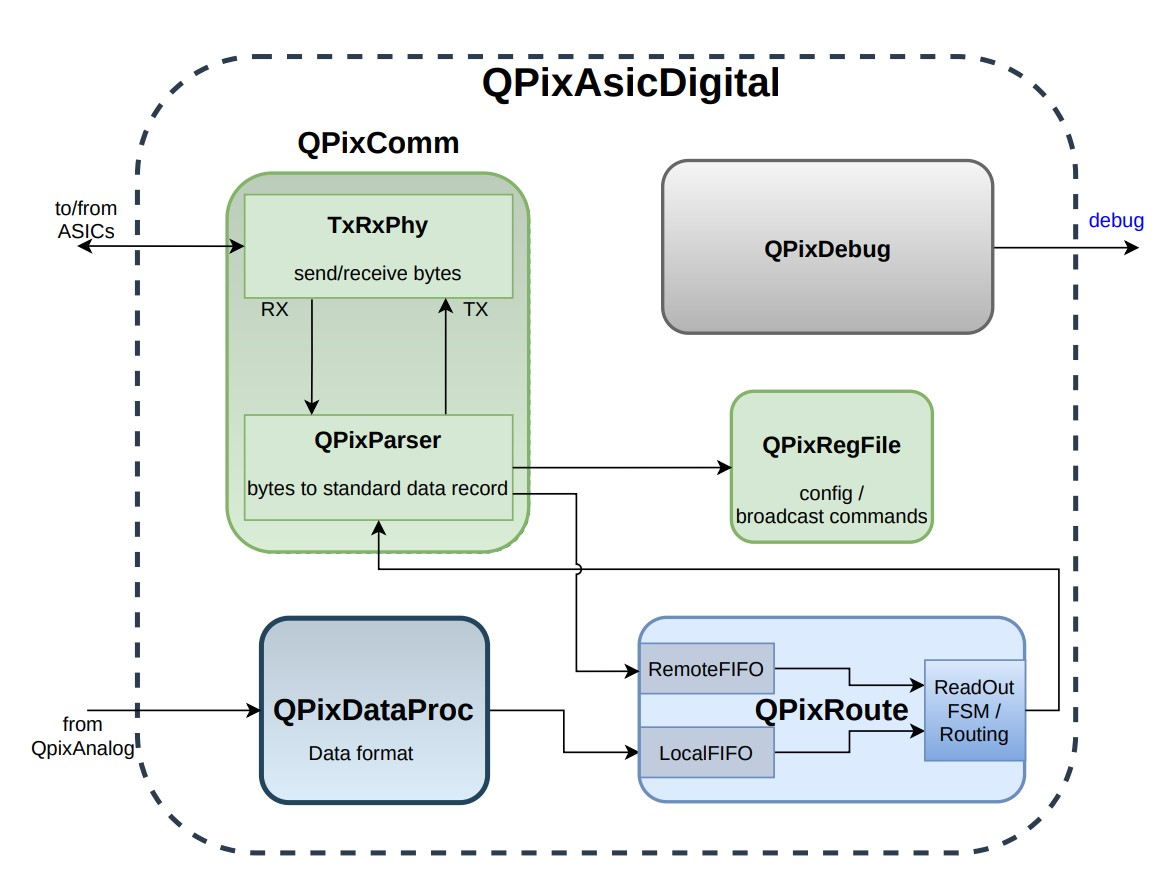
\includegraphics[width=\textwidth]{images/digital_node_overview.jpg}
\caption{Diagram of the Digital node.}
\end{figure}

Each of these remote ASICs are running on free-running independent clocks, with an expected frequency of $\approx$ 30 MHz.

\subsection{Basic System Requirements}

The sheer number of pixels required for an APA (and the entire module) require an effective means of charge and time calibration, stable buffer depths, and protection against single-point failure (SPF).
Resets are records of a local counter at the current node and are recorded in response to a reset pulse sent from a pixel.

\subsection{Frequency Calibration of each Node}

\subsection{Charge Calibration of each Pixel}~\label{sec:charge_calibration}

Natural decay products produced by $^{39}$Ar provide a continous source of incoming current across a LArTPC.

\subsubsection{Inter-Node communication via endeavor protocol}
~\label{sect:endeavor}

The Endeavor protocol is a bi-directional serial communication protocol which allows communication between asynchronous devices.
The asynchronous communication is achieved by extending the length of time that each bit is sent between the two devices.
In this protocol the way that the receiving node (RXN) identifies the correct logic value of the current bit is by counting the number of clocks that the incoming signal is logic high.
The incoming bit is either a logic low, if held high for fewer clocks than it would be if it was an incoming logic high.
The number of clocks which corresond to high and low must be programmed beforehand and are tunable parameters.

\subsubsection{The Structure of a Data Word}

Each node responds to a successful transmission of a 64-bit packet.
We choose that each packet, regardless of type, be 64-bits to reduce the overall packet checking complexity on each node.
The type of the packet then is selected by the word type, which is reserved for a static 4 bits within each 64-bit word.
This allows for a total amount of 16 unique packets each of which may be handled differently.

A successful transmission of a data word is indicated by the protocol when the correct number of bits have been read~(see Section~\ref{sect:endeavor}).
When a correct packet is filled a single flag is raised to indicate that the word is valid, and then the appropriate logic parses the header bits of the packet and determines how the packet should be handled.

There are two main types of packets that a digital node would receive, a register request or a data word from another node.
In the first case, the register request indicates that this packet originated from the aggregator node and may either to a specific node or a broadcast to the entire array.
Whether or not the register request is a broadcast is checked against another bit, and the packet is handled accordingly.
If the packet is a broadcast, the receiving node records an identification number associated with the broadcast, which it uses to ignore additional packets it may receive that correspond to the same broadcast.

The second kind of packet the digital node may receieve is a data type word.
In the case of data words, there are also two main types: a word which contains the 32 bit timestamp or an event end word.
The 32 bit timestamp data word are the words which must eventually make it to disk for analysis.
The data words must also encode the row and column position of the original nodes.

The event end words perform multiple functions.
First, they may used as checksums to indicate at the aggregator node, or on disk, that this node has successfully transmitted all of its data.
Secondly, the event end word, since it is necessarily 64 bits long, may also transmit its own timestamp with the excess bits.
The timestamp that the event end word carries is the time that the time that the node received the broadcast.
This timestamp is used in the frequency calibration of the node; the method for calibration is described in greater detail in Section~\ref{sec:calib}.


\begin{figure}[]
\centering
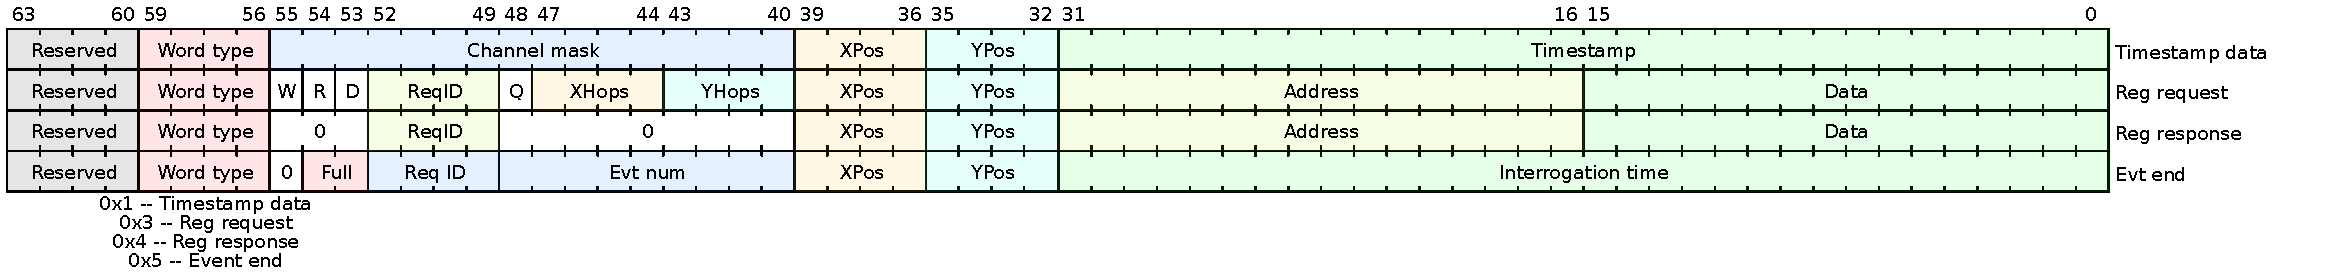
\includegraphics[width=\textwidth]{images/qpix_word_format.pdf}
\caption{Example of Datum words and their allocation as currently implemented in the simulation and first prototypes.}
\end{figure}~\label{fig:datum}

\subsubsection{Comments on Data Rates and required Computing}

Based on the minimum number of bits for each RTD~\ref{bit_calc} we can estimate minimum data rates based on tile size.


\section{The Digital Finite State Machine}

The Finite State Machine (FSM) of the remote digital ASIC outlines the designed behavior response to inputs from a controlling DAQ node.

\begin{figure}[]
\centering
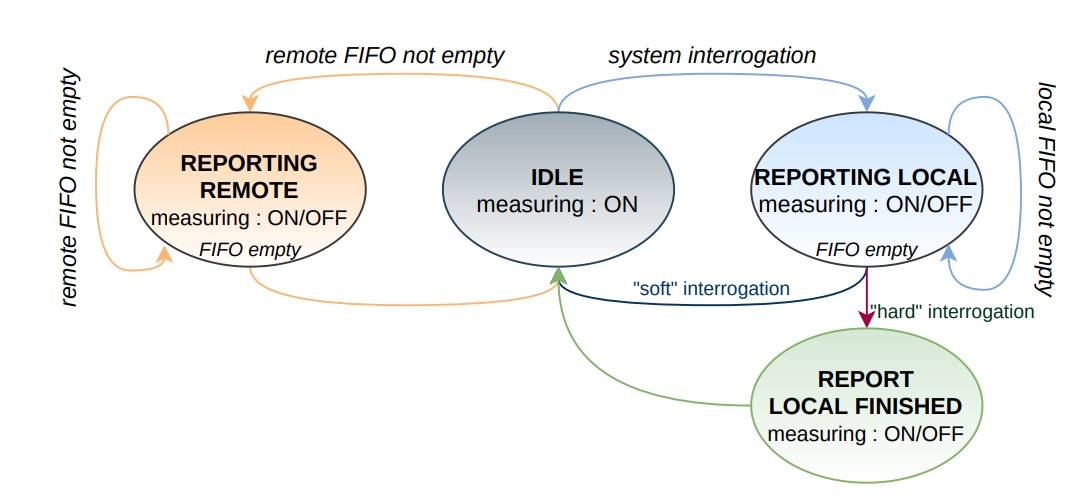
\includegraphics[width=\textwidth]{images/digital_fsm_overview.jpg}
\caption{Diagram of the Digital node's FSM which determines how to respond to incoming packets.}
\end{figure}

\begin{itemize}
    \item Idle, Acquisition State
    \item Transmit Local
    \item Transmit Finish
    \item Transmit Remote
    \item DONE
\end{itemize}
\label{fsm_state_labels}

\section{The Parameter Space of the Digital System}

The digital back-end design

\subsection{Buffer Depth Requirements}

The required buffer depth of each node in an array is the maximum number of timestamps the node can store in memory before overflow (dataloss).
Each node requires some buffer memory to record local data as well as separate storage for remote data.
The remote data which can be sent can come from any of the adjacent connected nodes, and may of any type: data words, register request, etc.
Since the remote

The ice40 FPGAs have a total of 20 Embedded Block Ram models (EBRs) which allow for a for total of 64xTODO memory depths allocated in each node.

\subsection{Endeavor Packet Stability at Different Scales}


\subsection{The Push and Pull Architectures}

%% QDB Hardware Discussion
\section{The Digital Prototype Design}

%% schematic of PCB

\section{Timing Stability}

We describe here the methods of measuring a stable time for different configurations of the nodes.
We also comment on the results of the timing with resepect to the minimum required timing sensitivity in order to have accurate timestamp reconstruction.

\section{Power and Current Characteristics}


\section{Analysis of Systematics for Different System Implementations}

The essential features of the digital node in the Q-Pix readout are the properties of the local oscillator.
The frequency, relative phases, and stability of the oscillator determine the power consumption, packet transaction time, minimum timestamp resolution, which determines maximum current measurements, and affects packet loss probability in larger tile systems.
It is not an understatement to say that the successful development of the digital node relies on the development of the local oscillator.

\section{Towards the Integration of the Aggregator Node}

In the studies presented here, The aggregator node which was used was the Zybo Z7-20.


\section{Comments on A Super-DAQ-Node}

Each APA module within a larger DUNE module must ultimately be interconnected so that the entire module can be readout.
As described above, a single modular tile is controlled by an individual DAQ node, where many constitute a complete APA.
Therefore, we refer to the device that digitally multiplexes all of the DAQ node data as the "Super DAQ Node" (SDN).
Then, we imagine the final multiplexing stage for an entire DUNE module as an array of SDNs, each of which consistute an array of DAQ nodes, where each DAQ node is a 2-D array of Q-Pix based ASICs.

The total number of request SDNs within the full dune module depends on the final size of a DAQ-node controlled tile.

%% high level figure here from TPC -> Integrator -> Digital Node -> Aggregator -> SuperDAQ-Node -> WIC -> Disc

\section{The Back-End Summary}
